\section{The Lifecycle of an Update Proposal}
An \emph{Update Proposal (UP)} is the unit of change for the blockchain software. It must have a clear goal of what it tries to achieve and why it would be beneficial if applied to the system. Moreover it should have a clear scope. In Figure \ref{lifecycle}, we depict the full lifecycle of an Update Proposal.

\begin{figure}[H]
    \caption{The Lifecycle of an Update Proposal (UP)}
    \centering
    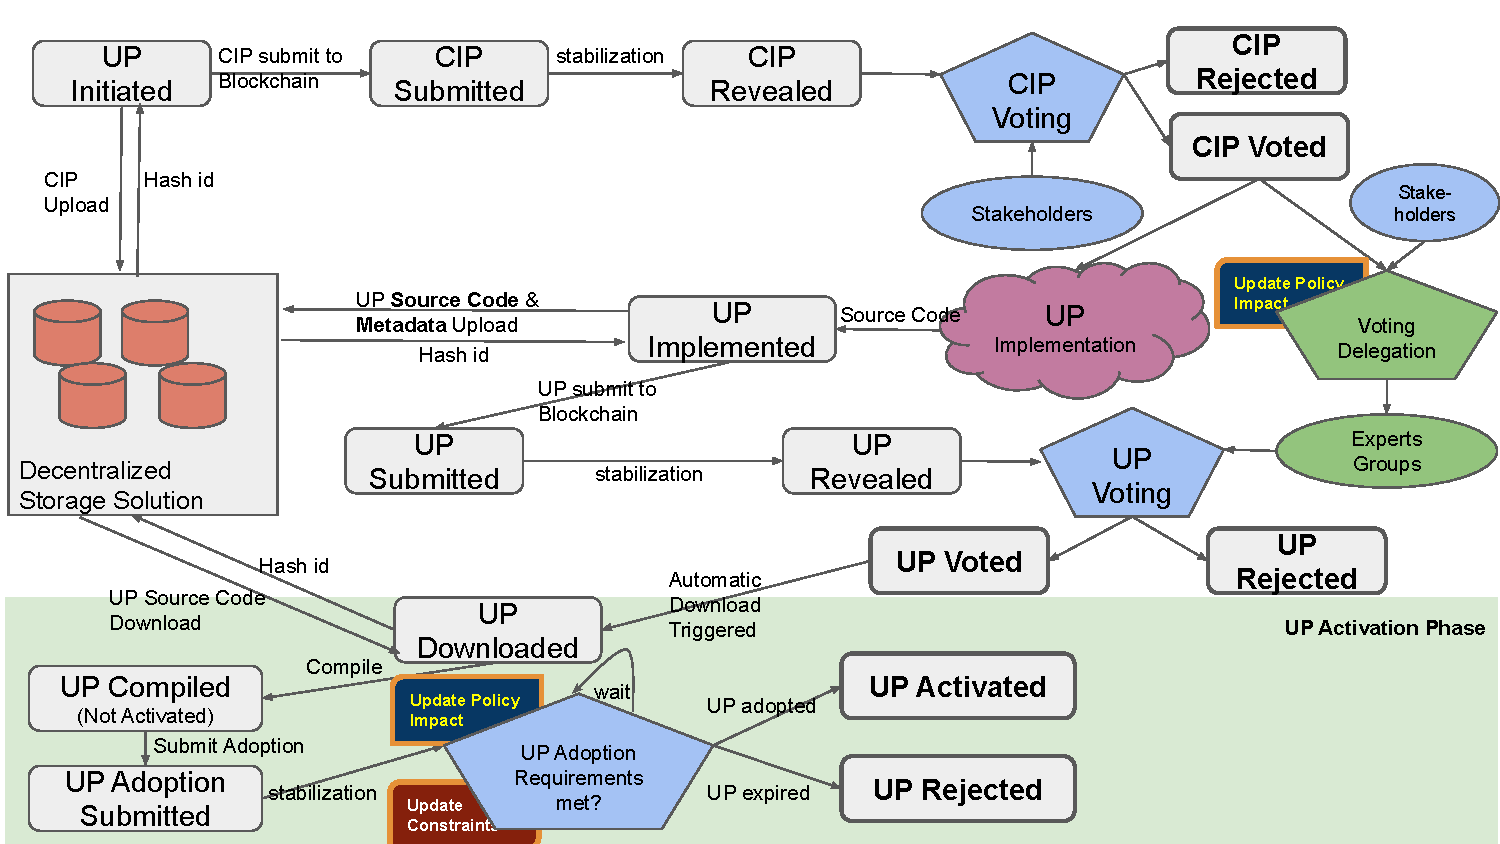
\includegraphics[width=0.9 \columnwidth,keepaspectratio]{figures/Update_Proposal_Lifecycle.pdf}
    \label{lifecycle}
\end{figure}

A UP starts its life as an idea for improvement of the blockchain system, which is recorded in a human readable simple text document, called the \emph{CIP}, which stands for \emph{Cardano Improvement Proposal}\footnote{We have used the Cardano \citep{cardano} blockchain system as an example of a stake-based ledger.}. A CIP includes basic information about a UP, such as the title, a basic description, the author(s) etc. Its sole purpose is to justify the necessity of the proposed software update and try to raise awareness and support from the community of users.

A CIP is initially uploaded to some external (to the blockchain system) decentralized storage solution\footnote{We will come back to this in the corresponding section} and a hash id is generated, in order to uniquely identify it. This hash id is committed to the blockchain in a two-step approach following a hash-based commitment scheme, in order to preserve the rightful authorship of the CIP.

Once the CIP is revealed a voting period for the specific proposal is initiated. Any stakeholder is eligible to vote for a CIP and the voting power will be proportional to his/her stake. Note that since a CIP is a document justifying the purpose and benefit of a proposed software update, it should not require in general sufficient technical expertise, in order for a stakeholder to review it and decide on his/her vote. A CIP after the voting period can either voted or rejected. Details on the voting protocol can be found in the relevant section.


